
\subsection*{Coulumb potential}

\fxnote{Introduce Coulumb}

First considering the value of $\rho_{max}$ in the case without a repulsive Coulumb interaction. Where finding a value of $\rho_{max}$ so that the eigenvalues are stable is the first step. \fxnote{rewrite sentence}  
%----------------------------------
\begin{wraptable}{r}{5.0cm}
\caption{hei hei} 
\label{tab:rhomax}
\phantom{.}
\begin{tabular}{|c|c|c|}
\hline
$\rho_{max}$ & N & 3rd eigenvalue \\
\hline 
1 & 10 & 83.5237 \\
2 & 20 & 21.8365 \\
3 & 30 & 9.79411 \\
4 & 40 & 5.5277 \\
\vdots & \vdots & \vdots \\
9 & 90 & 1.0983 \\
10 & 100 & 0.890899 \\
10.1 & 101 & 0.873488 \\
11 & 110 & 0.737631 \\
\hline

\end{tabular}

\end{wraptable}
%------------------------------------
Stable is chosen so that the values doesn't change to much. This is in the area of $\rho_{max} = 10$ and the change is about 0.2 between the surrounding steps. Also the change between 10 and 10.1 is about 0.02 so small changes in $\rho_{max} $ doesn't give big changes. Also the relation between $\rho_{max}$ and n is kept constant so that \fxnote{ref h} is constant. Running for different values of $\rho_{max}$ with the ratio gives \tabref{tab:rhomax}, which shows that when $\rho_{max} $ is 10 the results are stable for the 3rd eigenvalue. The reason for choosing the 3rd eigenvalue is that it is more sensitive for change of $\rho_{max}$ and it's the last printed eigenvalue in the program. 


Write smt awesomeabout the following plot of the eigenfunctions :D

\begin{figure}[H]
	\centering
	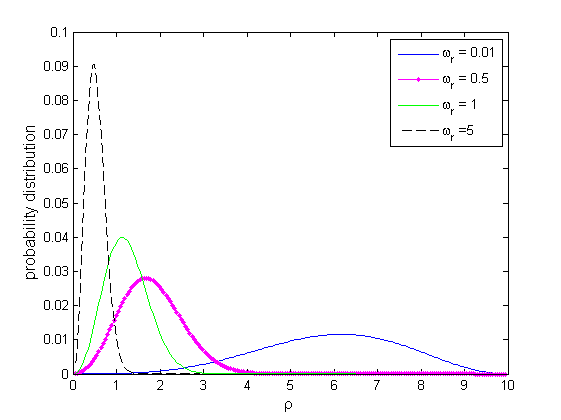
\includegraphics[width=0.75\textwidth]{Figures/ProbFuncOmega.png}
	\caption{Awesome caption}
	\label{fig:ProbFuncOmega}
\end{figure}





